\documentclass[aspectratio=169]{beamer}

\usepackage{emoji}
\usepackage{pgfplots}
\usepackage{tikz}
\usepackage{xcolor}

\usetikzlibrary{arrows.meta}
\usetikzlibrary{calc}
\usetheme{UiO}

\title{Kunstig intelligens}
\subtitle{Hva er det, og hvilke muligheter åpnes?}
\date{27.11.2024}
\author{Esten H. Leonardsen}

\setbeamertemplate{itemize/enumerate body begin}{\small}
\setbeamertemplate{itemize/enumerate subbody begin}{\footnotesize}

\begin{document}
    \begin{frame}
        \titlepage
    \end{frame}

    \begin{frame}{Oversikt}
        \begin{columns}
            \begin{column}{0.3\textwidth}
            \end{column}
            \begin{column}{0.7\textwidth}
                \begin{enumerate}
                    \item Kunstig intelligens
                    \begin{itemize}
                        \item Historikk, definisjoner, terminologi
                    \end{itemize}
                    \item Hvilke muligheter åpnes?
                    \item Praktiske erfaringer
                \end{enumerate}
            \end{column}
        \end{columns}
    \end{frame}

    \begin{frame}{Kunstig intelligens}
        \begin{columns}
            \begin{column}{0.3\textwidth}
            \end{column}
            \begin{column}{0.7\textwidth}
                \begin{tikzpicture}
                    \node[] at (-4.5, -3.25) {};
                    \node[] at (4.5, 3.25) {};

                    \visible<1-4>{
                        \node[anchor=north, align=center, font=\small\bfseries\linespread{0.9}\selectfont] at (0, 3.15) {Kunstig\\intelligens};
                    }
                    \visible<2>{
                        \node[anchor=north, inner sep=0pt, draw=black, label=below:{\small{Alan Turing}}] at (0, 1.5) {
                            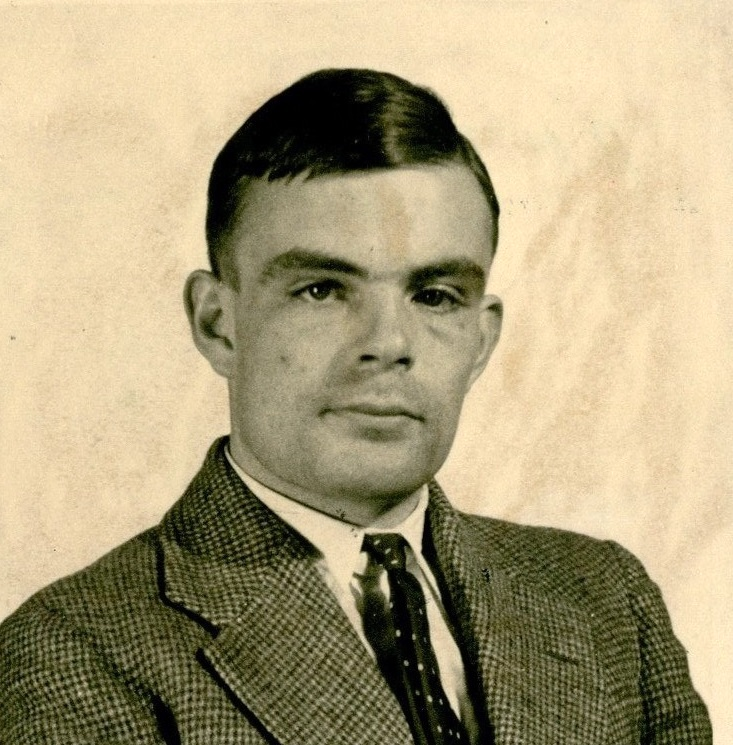
\includegraphics[width=4cm]{data/turing.jpeg}
                        };
                    }
                    \visible<3>{
                        \node[anchor=north, inner sep=0pt, draw=black] (thinking) at (0, 1.5) {
                            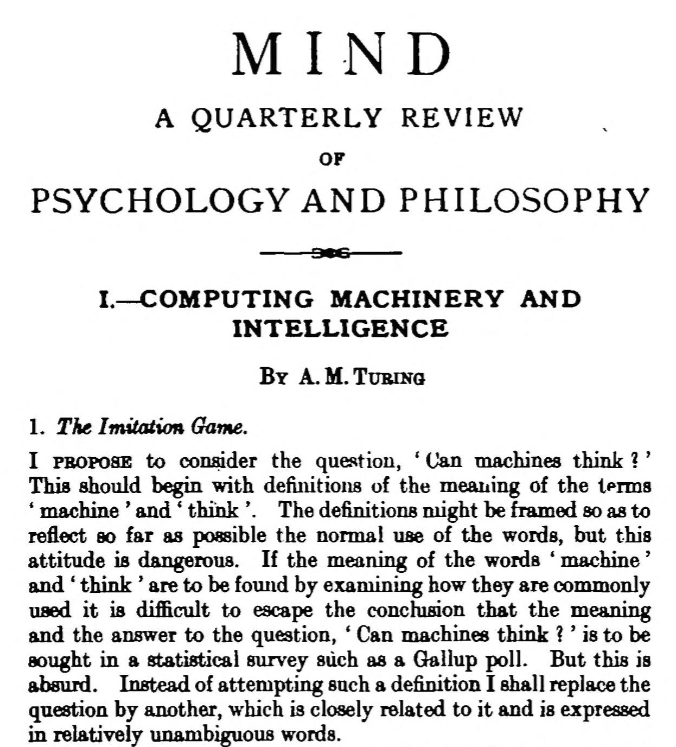
\includegraphics[width=3.75cm]{data/thinking.png}
                        };

                        \node[very thick, draw=red, minimum width=1.37cm, minimum height=0.08cm, anchor=east] at ($ (thinking.east)  - (0.092, 0.47) $) {};
                    }
                    \visible<4>{
                        \node[anchor=south, text width=6.5cm, font=\small\linespread{0.9}\selectfont, align=center] at (0, -3.35) {
                            Teknologi som løser oppgaver som\\krever en eller annen form for\\menneskelig intelligens
                        };
                    }

                    \visible<5,8,11-12,14>{
                        \node[circle, fill=blue!60, minimum size=5cm, anchor=north] (ai) at (0, 3.25) {};
                        \node[white, anchor=north, align=center, font=\small\bfseries\linespread{0.9}\selectfont] at ($ (ai.north) - (0, 0.1) $) {Kunstig\\intelligens};
                    }
                    \visible<5>{
                        \node[anchor=south, text width=6.5cm, font=\small\linespread{0.9}\selectfont, align=center] at (0, -3.35) {
                            Et fagfelt som produserer teknologi som løser oppgaver som krever en eller annen form for menneskelig intelligens
                        };
                    }

                    \visible<6-7,9-10,13>{
                        \node[label=below:\footnotesize{Input}, anchor=west, inner sep=0pt, outer sep=0pt] (input) at (-3.5, 0) {
                            \Huge{\emoji{spiral-notepad}}
                        };
                        \node[draw=black, label=below:\footnotesize{Prediksjon}, anchor=east] (output) at (3.5, 0) {
                            \footnotesize{Influensa}
                        };
                    }
                    \visible<6-7>{
                        \node[draw=black, dashed, minimum width=2.75cm, minimum height=2cm, label=above:\small{Ekspertsystem}] (system) at ($ (input.east)!0.5!(output.west) $) {};
                    }

                    \visible<6-7,9-10,13>{
                        \draw[-stealth] (input.east) -- (system.west);
                        \draw[-stealth] (system.east) -- (output.west);
                    }
                    \visible<7>{
                        \node[dotted, draw=black, minimum width=1.5cm] (s1) at ($ (system) + (0, 0.6) $) {
                            \scriptsize{Har feber}
                        };
                        \node[dotted, draw=black, minimum width=1.5cm] (s2) at (system) {
                            \scriptsize{Hoster}
                        };
                        \node[dotted, draw=black, minimum width=1.5cm] (s3) at ($ (system) - (0, 0.6) $) {
                            \scriptsize{Sår hals}
                        };

                        \draw[-] (system.west) -- (s1.west);
                        \draw[-] (system.west) -- (s2.west);
                        \draw[-] (system.west) -- (s3.west);

                        \draw[-] (s1.east) -- (system.east);
                        \draw[-] (s2.east) -- (system.east);
                        \draw[-] (s3.east) -- (system.east);

                        \node[] (expert) at ($ (system.south) - (0, 1.75) $) {
                            \Huge{\emoji{woman-scientist}}
                        };
                        \draw[-stealth, line width=4pt, gray!75] (expert) -- (system);
                    }

                    \visible<8,11-12,14>{
                        \node[circle, fill=purple!60, anchor=south, minimum size=3.7cm] (ml) at ($ (ai.south) + (0, 0.05) $) {};
                        \node[white, anchor=north, align=center, font=\small\bfseries\linespread{0.9}\selectfont] at ($ (ml.north) - (0, 0.3) $) {Maskinlæring};
                    }
                    \visible<9-10>{
                        \node[draw=black, dashed, minimum width=2.75cm, minimum height=2cm, label=above:\small{Maskinlæringsmodell}] (system) at ($ (input.east)!0.5!(output.west) $) {};
                    }
                    \visible<10>{
                        \node[] at (system) {
                            
\includegraphics[width=2.5cm]{data/cogwheels.png}
                        };
                    }
                    \visible<11>{
                        \node[anchor=south, text width=6.5cm, font=\small\linespread{0.9}\selectfont, align=center] at (0, -3.35) {
                            Teknologi som lærer seg å løse\\oppgaver ved å finne mønstre i treningsdata
                        };
                    }

                    \visible<12,14>{
                        \node[circle, fill=red!60, anchor=south, minimum size=2.5cm] (dl) at ($ (ml.south) + (0, 0.05) $) {};
                        \node[white, anchor=north, align=center, font=\small\bfseries\linespread{0.9}\selectfont] at ($ (dl.north) - (0, 0.1) $) {Dyp\\læring};
                    }
                    \visible<13>{
                        \node[draw=black, dashed, minimum width=2.75cm, minimum height=2.1cm, label=above:\small{Kunstig nevralt nettverk}] (system) at ($ (input.east)!0.5!(output.west) $) {};

                        \node[circle, minimum width=0.4cm, fill=teal!60] (n00) at ($ (system) + (-0.75, 0.75) $) {};
                        \node[circle, minimum width=0.4cm, fill=teal!60] (n01) at ($ (system) + (-0.75, 0.25) $) {};
                        \node[circle, minimum width=0.4cm, fill=teal!60] (n02) at ($ (system) - (0.75, 0.25) $) {};
                        \node[circle, minimum width=0.4cm, fill=teal!60] (n03) at ($ (system) - (0.75, 0.75) $) {};

                        \node[circle, minimum width=0.4cm, fill=teal!60] (n10) at ($ (system) + (0, 0.5) $) {};
                        \node[circle, minimum width=0.4cm, fill=teal!60] (n11) at (system) {};
                        \node[circle, minimum width=0.4cm, fill=teal!60] (n12) at ($ (system) - (0, 0.5) $) {};

                        \node[circle, minimum width=0.4cm, fill=teal!60] (n20) at ($ (system) + (0.75, 0.25) $) {};
                        \node[circle, minimum width=0.4cm, fill=teal!60] (n21) at ($ (system) - (-0.75, 0.25) $) {};

                        \draw[] (system.west) -- (n00);
                        \draw[] (system.west) -- (n01);
                        \draw[] (system.west) -- (n02);
                        \draw[] (system.west) -- (n03);

                        \draw[] (n00) -- (n10);
                        \draw[] (n00) -- (n11);
                        \draw[] (n00) -- (n12);
                        \draw[] (n01) -- (n10);
                        \draw[] (n01) -- (n11);
                        \draw[] (n01) -- (n12);
                        \draw[] (n02) -- (n10);
                        \draw[] (n02) -- (n11);
                        \draw[] (n02) -- (n12);
                        \draw[] (n03) -- (n10);
                        \draw[] (n03) -- (n11);
                        \draw[] (n03) -- (n12);

                        \draw[] (n10) -- (n20);
                        \draw[] (n10) -- (n21);
                        \draw[] (n11) -- (n20);
                        \draw[] (n11) -- (n21);
                        \draw[] (n12) -- (n20);
                        \draw[] (n12) -- (n21);

                        \draw[] (n20) -- (system.east);
                        \draw[] (n21) -- (system.east);
                    }

                    \visible<14>{
                        \node[anchor=east, white] at ($ (dl.east) - (0.3, 0.1) $) {GPT};
                        \node[anchor=west, white] at ($ (dl.west) - (-0.5, 0.7) $) {Dall-E};
                    }


                    \visible<14>{
                        \node[anchor=south, text width=6.5cm, font=\small\linespread{0.9}\selectfont, align=center] at (0, -3.35) {
                            Kunstige nevrale nettverk som lærer komplekse sammenhenger\\mellom input og output
                        };
                    }
                \end{tikzpicture}
            \end{column}
        \end{columns}
    \end{frame}

    \begin{frame}{Terminologi}
        \begin{columns}
            \begin{column}{0.3\textwidth}
            \end{column}
            \begin{column}{0.7\textwidth}
                \begin{tikzpicture}
                    \node[] at (-4.5, -3.25) {};
                    \node[] at (4.5, 3.25) {};

                    \only<1>{
                        \draw[dashed] (-4.5, 0) -- (4.5, 0);

                        \node[anchor=south east] at (4.5, 0) {
                            Veiledet
                        };

                        \node[label=below:{\scriptsize{Katt}}, inner sep=0pt, draw=black] at (-3, 2) {
                            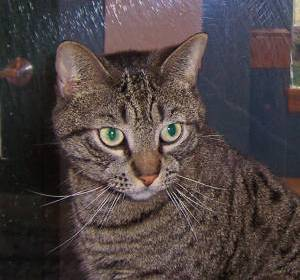
\includegraphics[width=1.5cm]{data/cat.1.jpg}
                        };
                        \node[label=below:{\scriptsize{Hund}}, inner sep=0pt, draw=black] at (-1, 2) {
                            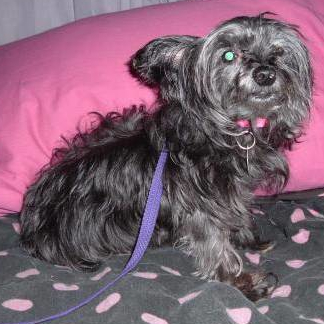
\includegraphics[width=1.5cm]{data/dog.0.jpg}
                        };
                        \node[label=below:{\scriptsize{Katt}}, inner sep=0pt, draw=black] at (1, 2) {
                            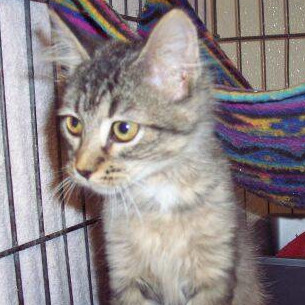
\includegraphics[width=1.5cm]{data/cat.2.jpg}
                        };
                        \node[label=below:{\scriptsize{Hund}}, inner sep=0pt, draw=black] at (3, 2) {
                            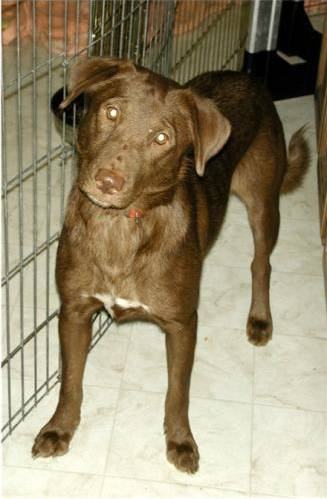
\includegraphics[width=1.5cm]{data/dog.1.jpg}
                        };

                        \node[anchor=north east] at (4.5, 0) {
                            Ikke-veiledet
                        };

                        \node[inner sep=0pt, draw=black] at (-3.25, -2.1) {
                            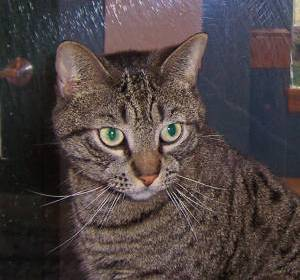
\includegraphics[width=1.25cm]{data/cat.1.jpg}
                        };
                        \node[inner sep=0pt, draw=black] at (-1.85, -1) {
                            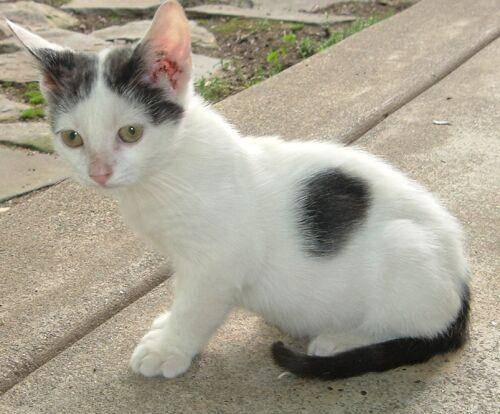
\includegraphics[width=1.25cm]{data/cat.3.jpg}
                        };
                        \node[inner sep=0pt, draw=black] at (-1.65, -2.5) {
                            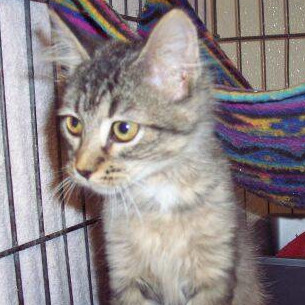
\includegraphics[width=1.25cm]{data/cat.2.jpg}
                        };
                        \node[inner sep=0pt, draw=black] at (-0.25, -1.25) {
                            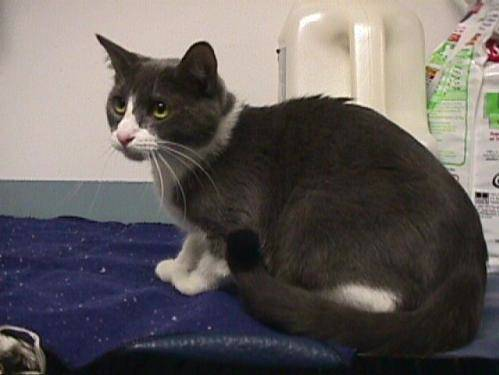
\includegraphics[width=1.25cm]{data/cat.4.jpg}
                        };

                        \node[inner sep=0pt, draw=black] at (2, -2.25) {
                            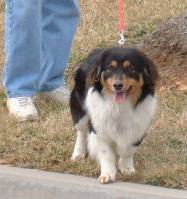
\includegraphics[width=1.25cm]{data/dog.2.jpg}
                        };
                        \node[inner sep=0pt, draw=black] at (3.55, -1.25) {
                            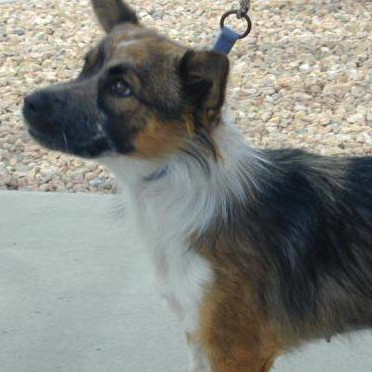
\includegraphics[width=1.25cm]{data/dog.3.jpg}
                        };
                        \node[inner sep=0pt, draw=black] at (3.65, -2.65) {
                            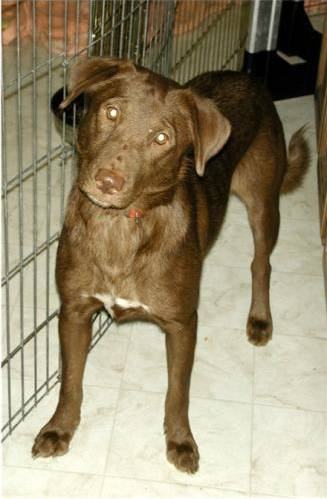
\includegraphics[width=1.25cm]{data/dog.1.jpg}
                        };
                        \draw[dashed, red, very thick] (1.1, -0.4) -- (0.6, -3.2);
                    }
                    \only<2>{
                        \node[anchor=south] at (0, -3.25) {
                            Forsterkende læring
                        };

                        \node[inner sep=0pt, draw=black] at (0, 0) {
                            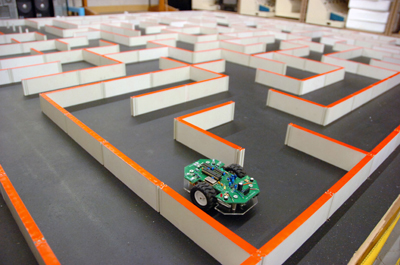
\includegraphics[width=6cm]{data/maze.jpg}
                        };
                    }
                    \only<3>{
                        \node[anchor=south] at (0, -3.25) {
                            Generativ kunstig intelligens
                        };

                        \node[inner sep=0pt, draw=black] at (0, 0) {
                            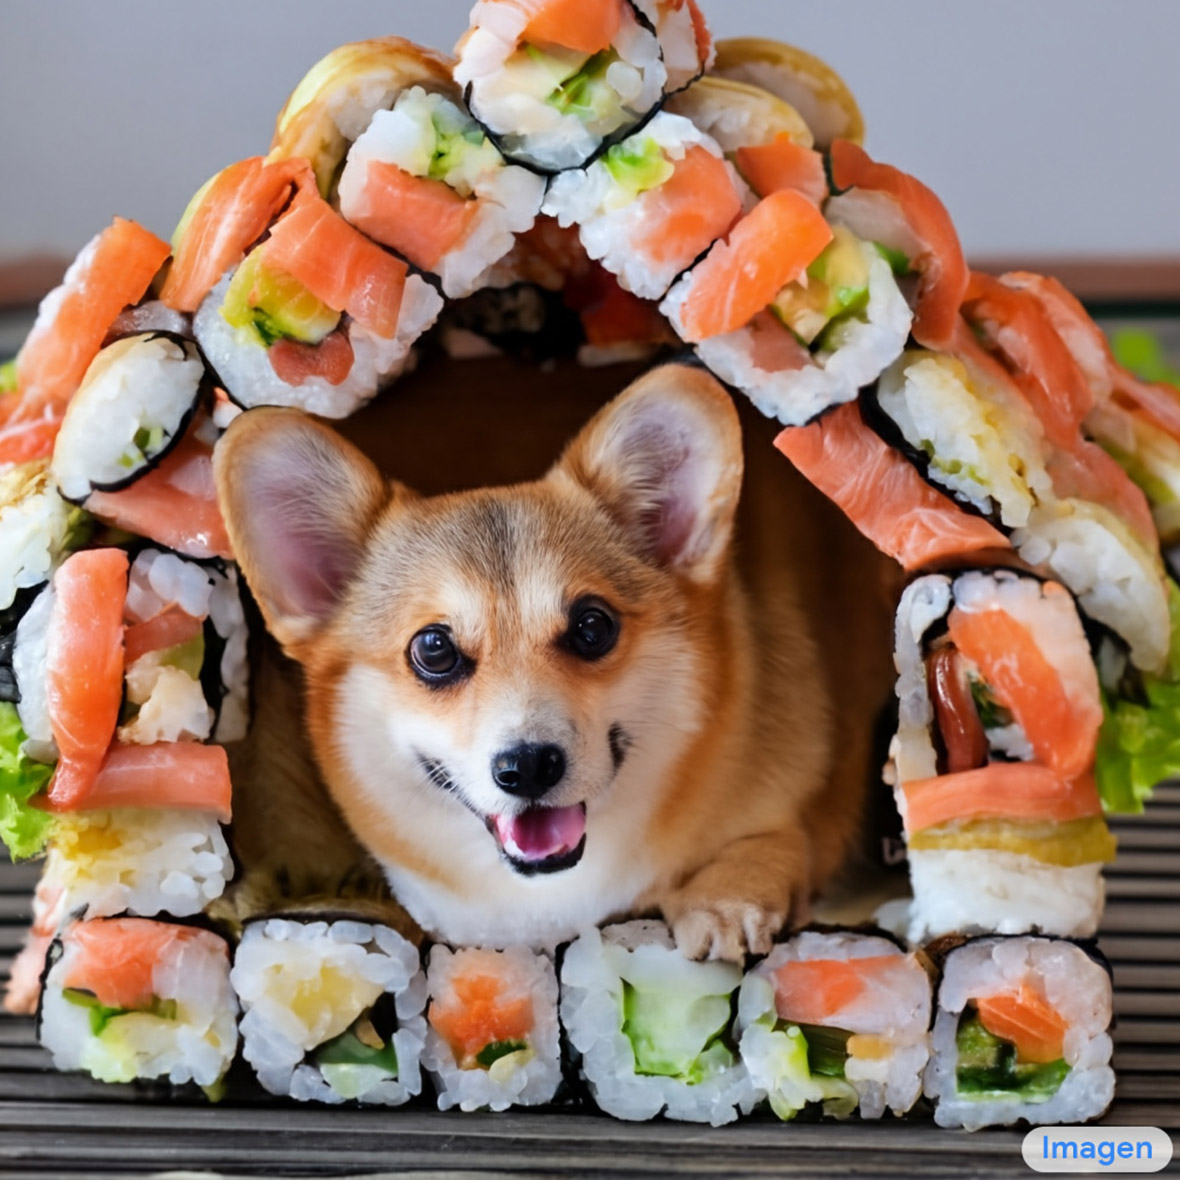
\includegraphics[width=4.5cm]{data/corgi.jpeg}
                        };
                    }
                    \only<4-7>{
                        \draw[stealth-stealth] (-4.25, -2.5) -- (4.25, -2.5);

                        \node[anchor=north west, font=\small\bfseries] at (-4.25, 3.15) {
                            Smal (svak)
                        };
                        \node[anchor=north east, font=\small\bfseries] at (4.25, 3.15) {
                            Generell (sterk)
                        };

                        \node[anchor=north west, font=\small] at (-4.25, -2.5) {
                            Mer spesifikk
                        };
                        \node[anchor=north east, font=\small] at (4.25, -2.5) {
                            Mer generell
                        };

                        \draw[-stealth, red] (-4, 2) -- (4, 2);
                        \node[anchor=north, align=center, text=red, text width=6.5cm, font=\small\linespread{0.9}\selectfont] at (0, 2) {I stand til å løse et større spekter problemer innen flere ulike domener};
                    }
                    \visible<5>{
                        \node[anchor=south east] at (4, -2.5) {
                            
\includegraphics[width=1cm]{data/human.png}
                        };
                        \node[anchor=south west] at (-4, -2.5) {
                            
\includegraphics[width=1cm]{data/laptop.png}
                        };
                    }
                    \visible<6-7>{
                        \node[align=center,font=\scriptsize, fill=blue!60, text=white, minimum width=1.8cm, rounded corners=.1cm] at (-3.25, -0.1) {
                            Bilde-\\
                            diagnostikk
                        };
                        \node[align=center,font=\scriptsize, fill=blue!60, text=white, minimum width=1.8cm, rounded corners=.1cm] at (-3.25, -1.05) {
                            Forsikrings-\\
                            prising
                        };
                        \node[align=center,font=\scriptsize, fill=blue!60, text=white, minimum width=1.8cm, rounded corners=.1cm] at (-3.25, -2) {
                            Dokument-\\
                            lesing
                        };
                    }

                    \visible<7>{
                        \node[align=center,font=\scriptsize, fill=blue!60, text=white, minimum width=1.8cm, rounded corners=.1cm] at (-0.5, -2) {
                            Selvkjørende\\biler
                        };
                        \node[align=center,font=\scriptsize, fill=blue!60, text=white, rounded corners=.1cm] at (0, -1.15) {
                            ChatGPT
                        };

                    }
                \end{tikzpicture}
            \end{column}
        \end{columns}
    \end{frame}

    \section{Mulighetsrom}

    \begin{frame}{Mulighetsrom}
        \begin{columns}
            \begin{column}{0.3\textwidth}
            \end{column}
            \begin{column}{0.7\textwidth}
                \begin{tikzpicture}
                    \visible<1>{
                        \node[anchor=north west, label=below:\small{Utforskende}, inner sep=0pt, draw=black] at (-4.25, 3) {
                            
\includegraphics[width=4.25cm]{data/exploratory.png}
                        };
                        \node[anchor=south east, label=below:\small{Automatiserende}, inner sep=0pt, draw=black] at (4.25, -2.75) {
                            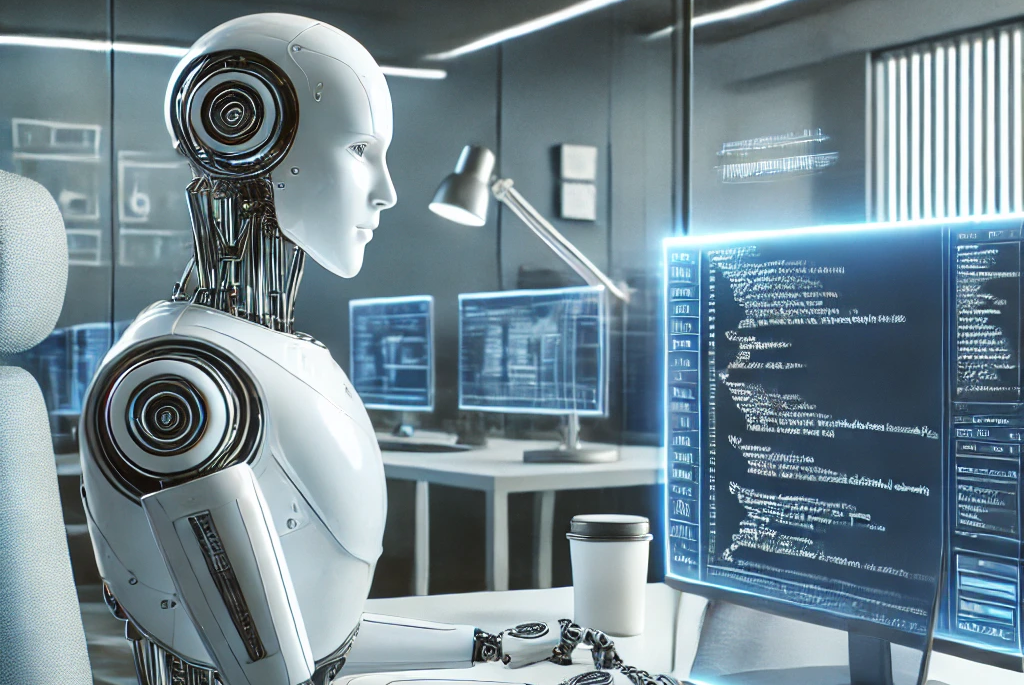
\includegraphics[width=4.25cm]{data/automation.png}
                        };
                    }

                    \visible<2->{
                        \node[anchor=south, text depth=0] at (-3, 1.2) {
                            Egenutvikling
                        };
                        \node[inner sep=0pt, draw=black] at (-3, 0) {
                            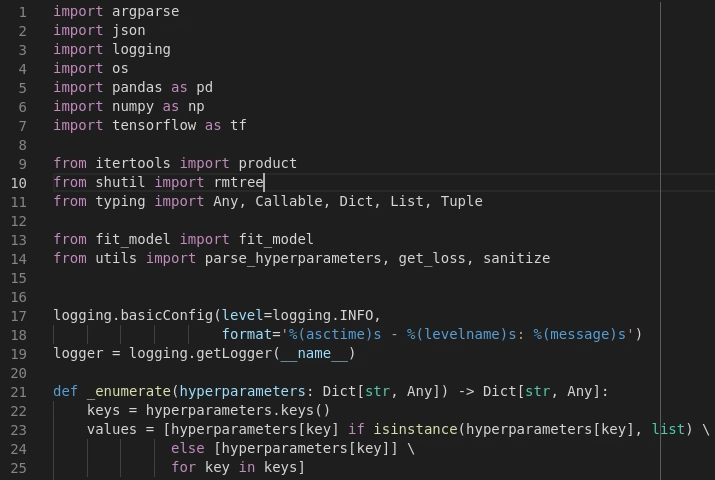
\includegraphics[width=2.5cm]{data/code.png}
                        };
                    }
                    \visible<3->{
                        \node[anchor=south, text depth=0] at (0, 1.2) {
                            Åpne modeller
                        };
                        \draw[dashed] (-1.5, 1.75) -- (-1.5, -1.75);
                        \node[inner sep=0pt, draw=black] at (0, 0) {
                            
\includegraphics[width=2.5cm]{data/huggingface.png}
                        };
                    }
                    \visible<4>{
                        \node[anchor=south, text depth=0] at (3, 1.2) {
                            Åpne APIer
                        };
                        \draw[dashed] (1.5, 1.75) -- (1.5, -1.75);
                        \node[inner sep=0pt, draw=black] at (3, 0) {
                            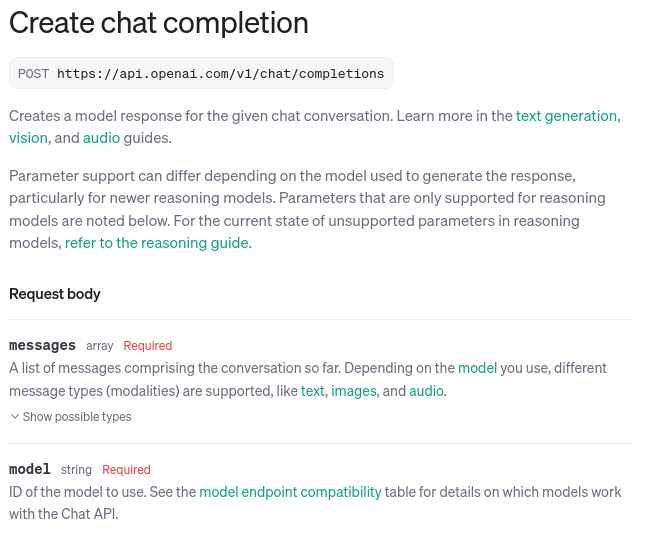
\includegraphics[width=2.5cm]{data/openai.png}
                        };
                    }

                \end{tikzpicture}
            \end{column}
        \end{columns}
    \end{frame}

    \section{Erfaringer}

    \begin{frame}{Erfaringer: Bilskade}
        \begin{columns}
            \begin{column}{0.25\textwidth}
            \end{column}
            \begin{column}{0.75\textwidth}
                \begin{tikzpicture}
                    \node[] at (-4.5, -3.25) {};
                    \node[] at (4.5, 3.25) {};

                    \visible<1>{
                        \node[] at (0, 0) {
                            \scalebox{-1}[1]{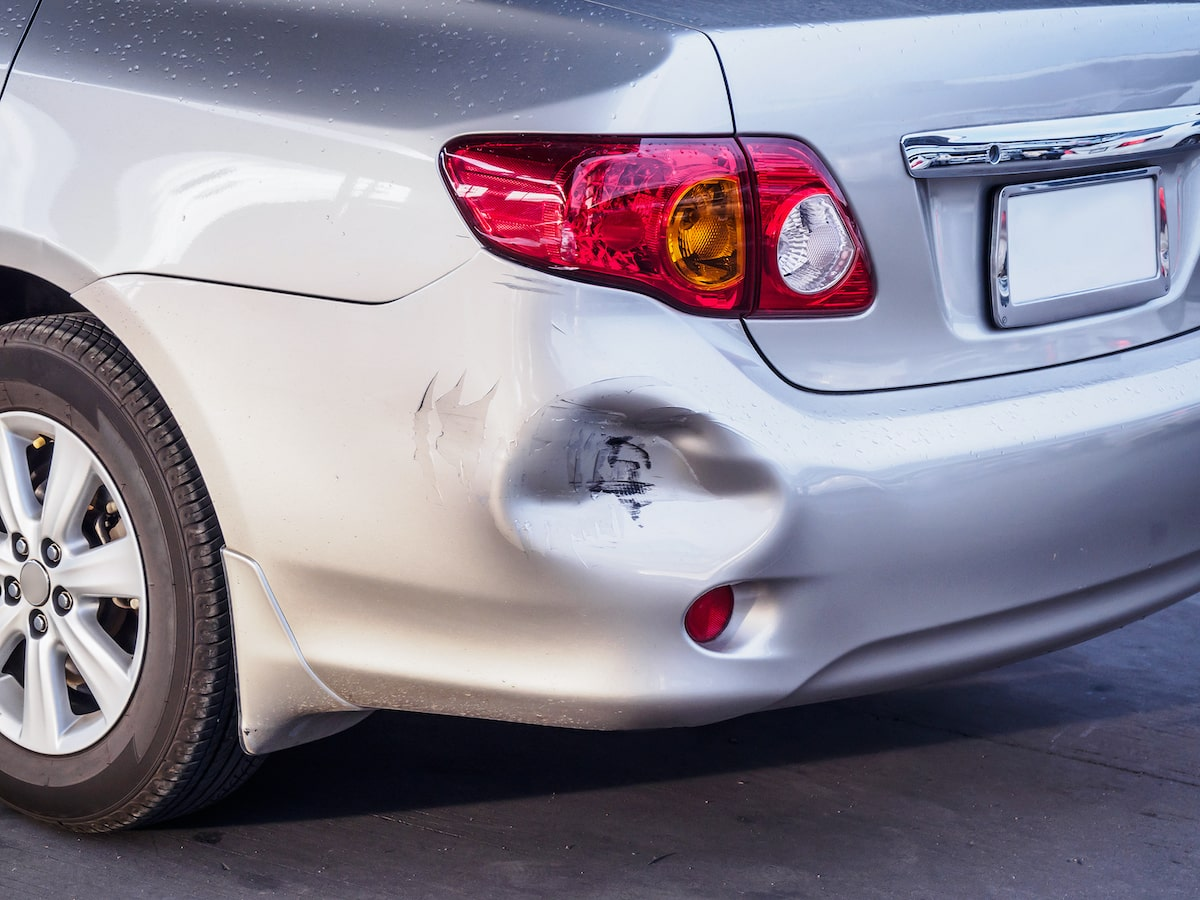
\includegraphics[width=6cm]{data/car1.jpg}}
                        };
                        \node[draw=red, very thick, minimum width=2cm, minimum height=1.5cm, label=below:{\textcolor{red}{25,000}}] at (0, -0.05) {};
                    }
                    \visible<2>{
                        \node[draw=black, inner sep=0pt, label=below:{\footnotesize{25,000}}] (car1) at (0, 2) {
                            \scalebox{-1}[1]{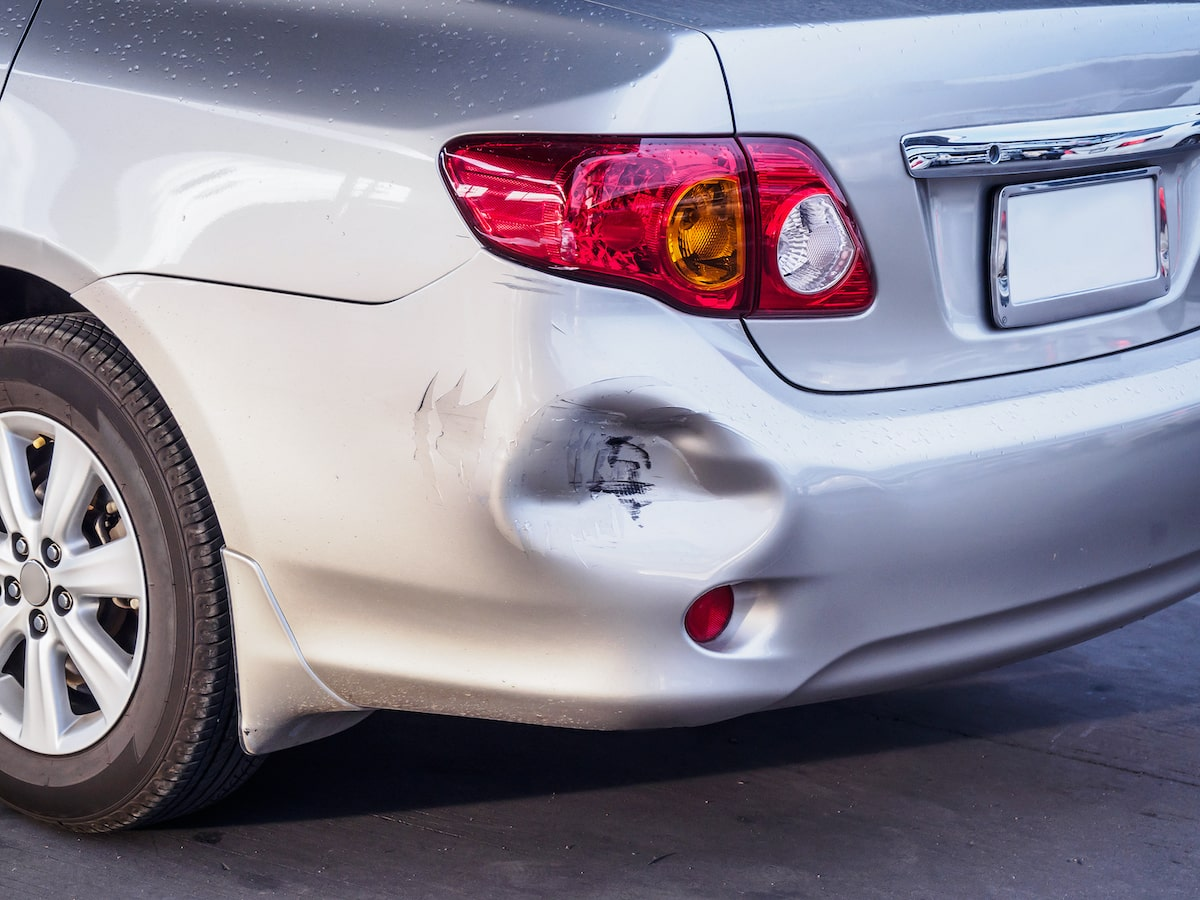
\includegraphics[width=1.75cm]{data/car1.jpg}}
                        };
                        \node[draw=black, inner sep=0pt, label=below:{\footnotesize{18,000}}] (car2) at (-2, 2) {
                            \scalebox{-1}[1]{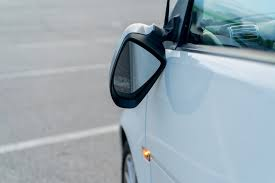
\includegraphics[width=1.75cm]{data/car2.jpeg}}
                        };
                        \node[draw=black, inner sep=0pt, label=below:{\footnotesize{12,000}}] (car3) at (2, 2) {
                            \scalebox{-1}[1]{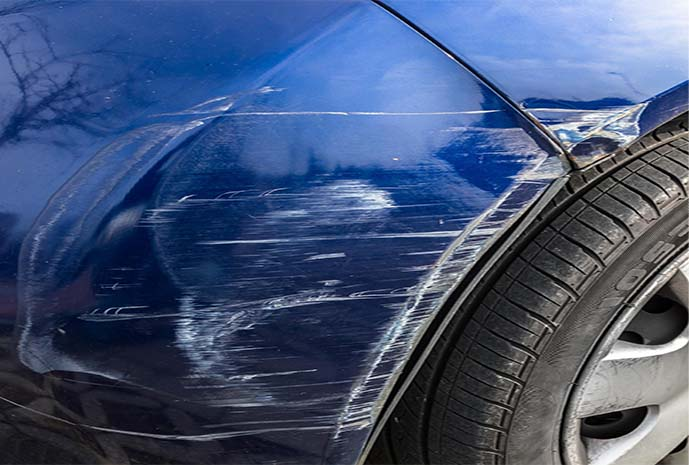
\includegraphics[width=1.75cm]{data/car3.jpg}}
                        };

                        \node[draw=black, dashed, label=below:{\small{Maskinlæringsmodell}}, minimum width=4cm, minimum height=2cm] (model) at (0, -1.75) {};

                        \draw[-stealth] ($ (car1.south) - (0, 0.4) $) -- (model);
                        \draw[-stealth] ($ (car2.south) - (0, 0.4) $) -- (model);
                        \draw[-stealth] ($ (car3.south) - (0, 0.4) $) -- (model);
                    }
                    \visible<3-4>{
                        \node[draw=black, inner sep=0pt] at (0, 0) {
                            \scalebox{-1}[1]{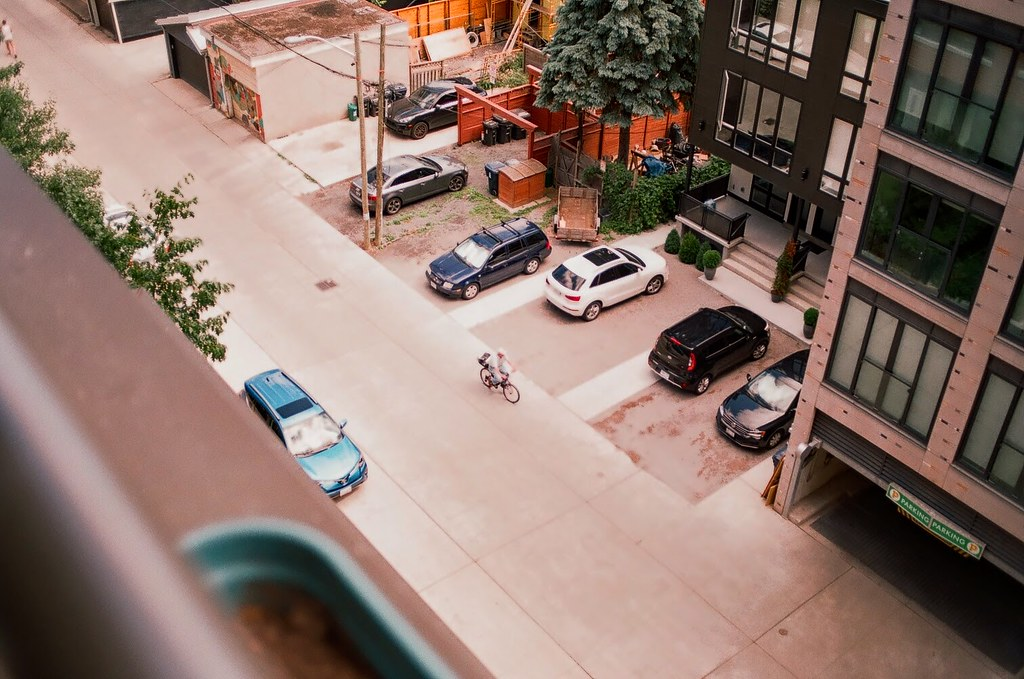
\includegraphics[width=5cm]{data/balcony.jpg}}
                        };
                    }
                    \visible<4>{
                        \node[circle, draw=red, thick, minimum size=0.7cm] at (-0.45, 0.3) {};
                    }
                    \visible<5>{
                        \node[anchor=west, align=left, text width=6.5cm] at (-3.25, 0) {
                            \textbf{Sørg for at data som kommer inn når systemet er satt i produksjon matcher treningsdataen!}
                            \begin{itemize}
                                \item Vurder om brukere trenger opplæring
                                \item Legg inn gode instruksjoner i sluttbrukerapplikasjonen
                            \end{itemize}
                        };
                    }
                \end{tikzpicture}
            \end{column}
        \end{columns}
    \end{frame}

    \begin{frame}{Erfaringer: Radiologi}
        \begin{columns}
            \begin{column}{0.25\textwidth}
            \end{column}
            \begin{column}{0.75\textwidth}
                \begin{tikzpicture}
                    \node[] at (-4.5, -3.5) {};
                    \node[] at (4.5, 3.5) {};

                    \visible<1>{
                        \node[draw=black, inner sep=0pt] at (0, 0) {
                            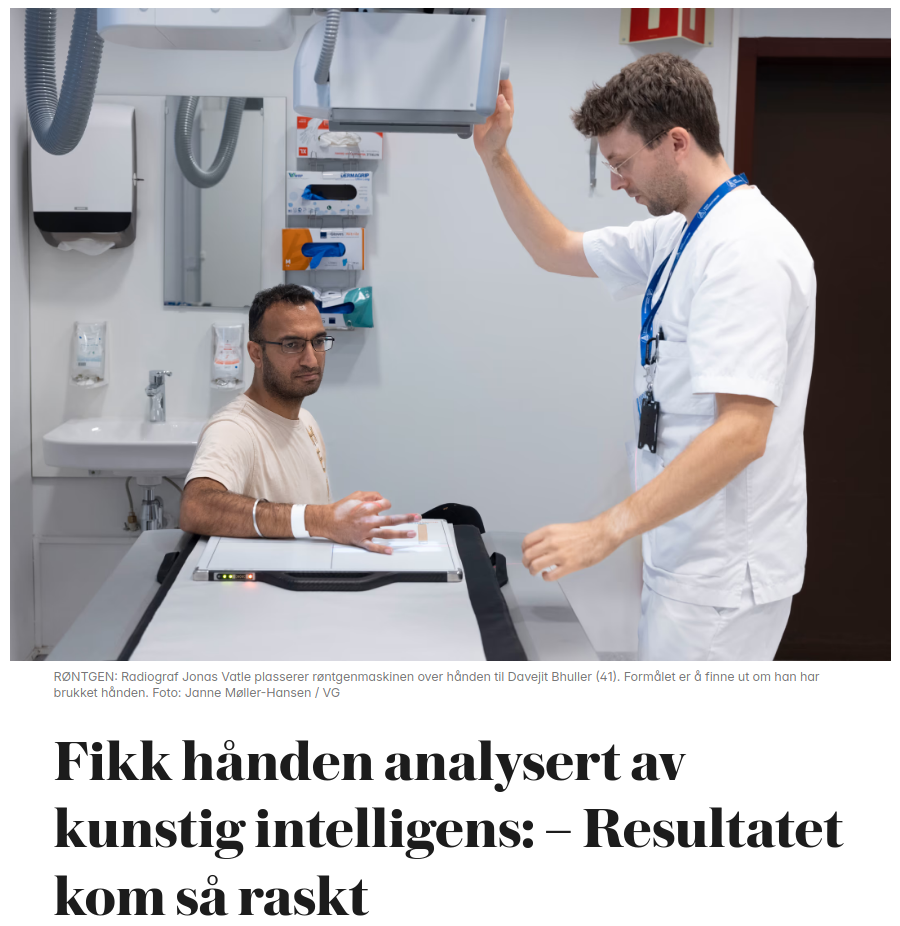
\includegraphics[width=6cm]{data/vg.png}
                        };
                    }
                    \visible<2>{
                        \node[draw=black, inner sep=0pt] at (0, 0) {
                            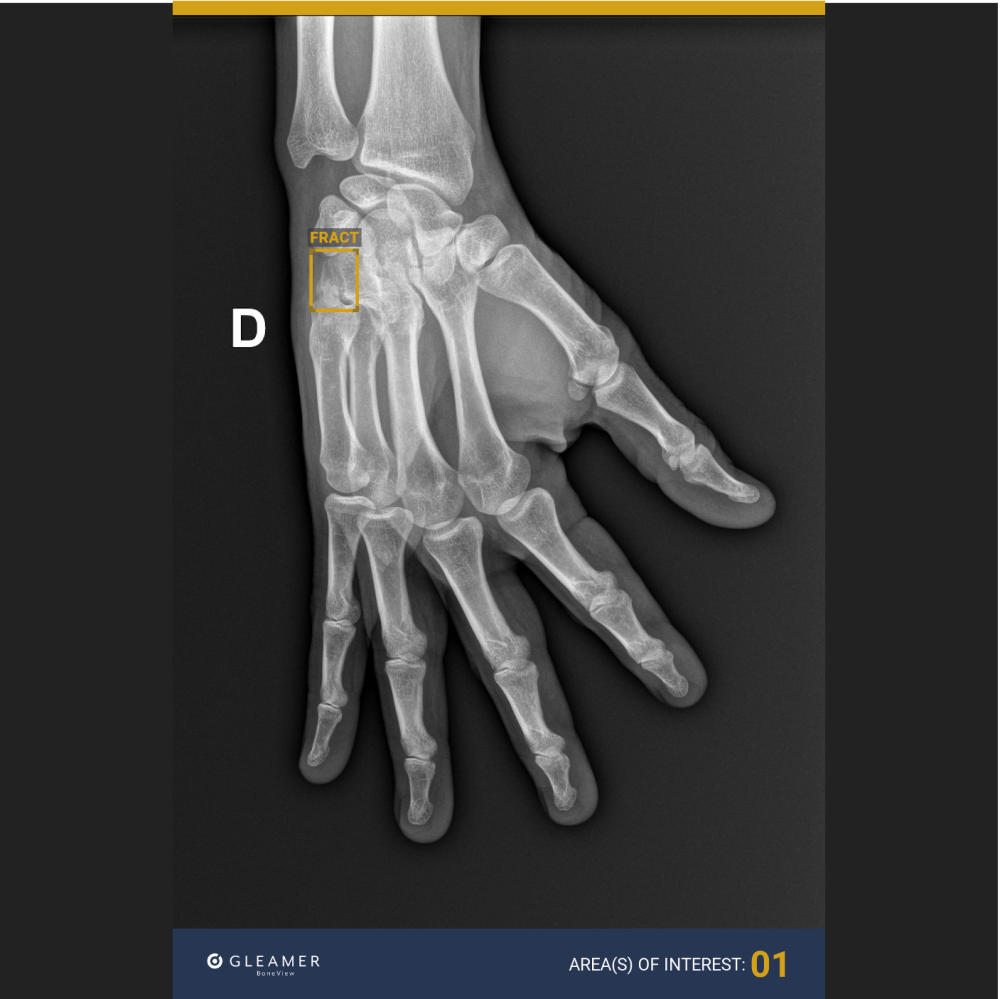
\includegraphics[width=5.5cm]{data/boneview.png}
                        };
                    }

                    \visible<3>{
                        \node[anchor=west, align=left, text width=6.5cm] at (-3.25, 0) {
                            \textbf{Sørg for at systemet som helhet}\\ \textbf{tolererer at prediksjonsmodellen tar feil!}
                            \begin{itemize}
                                \item Tving modellen til å uttrykke usikkerhet
                                \item Bruk menneskelige eksperter som et sikkerhetsnett
                            \end{itemize}
                        };
                    }
                \end{tikzpicture}
            \end{column}
        \end{columns}
    \end{frame}

    \begin{frame}{Erfaringer: Bildeanalyse}
        \begin{columns}
            \begin{column}{0.25\textwidth}
            \end{column}
            \begin{column}{0.75\textwidth}
                \begin{tikzpicture}
                    \node[] at (-4.5, -3.5) {};
                    \node[] at (4.5, 3.5) {};

                    \visible<1>{
                        \node[] at (0, 0) {
                            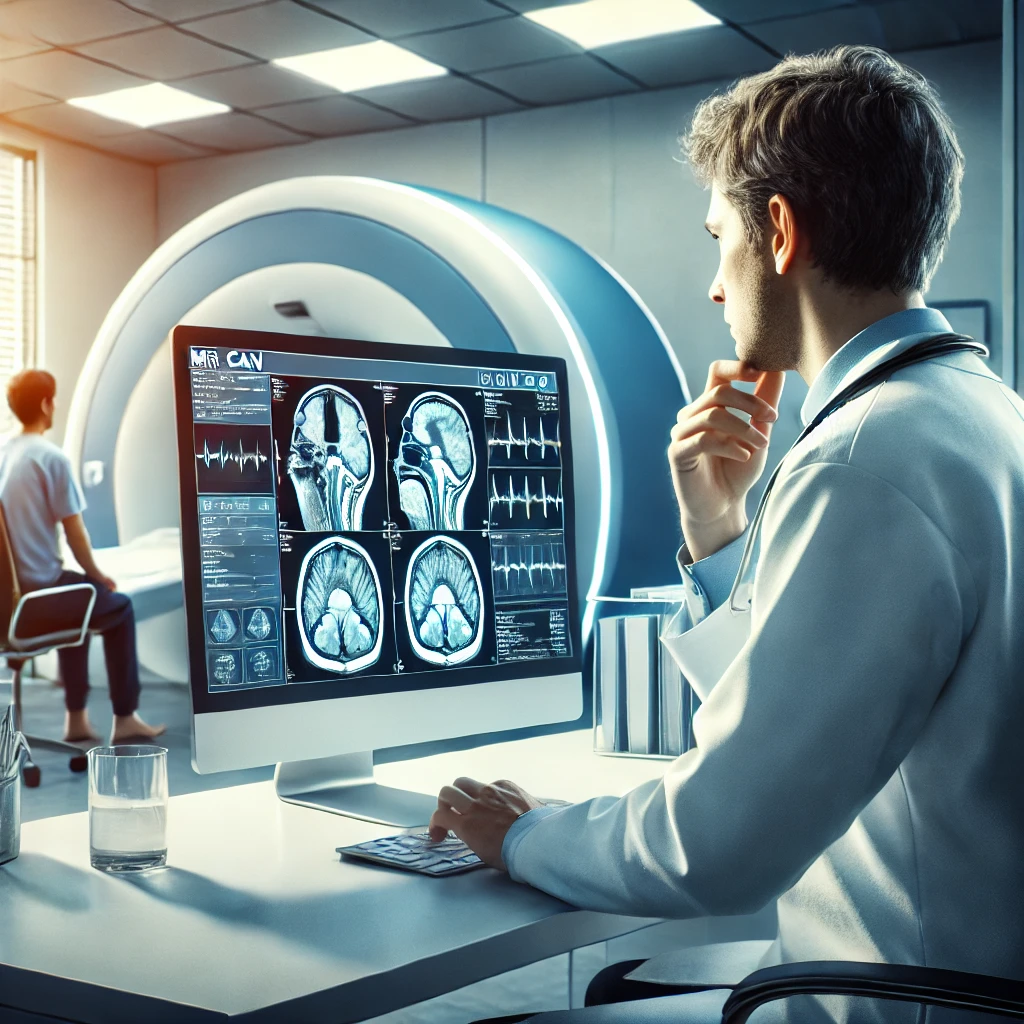
\includegraphics[width=6cm]{data/doctor.png}
                        };
                    }
                    \visible<2>{
                        \node[anchor=west, align=left, text width=6.5cm] at (-3.25, 0) {
                            \textbf{Bruk menneskelige eksperter i utviklingsarbeidet!}
                            \begin{itemize}
                                \item Sørg for at modellen har tilgang til tilstrekkelig informasjon
                            \end{itemize}
                        };
                    }
                \end{tikzpicture}
            \end{column}
        \end{columns}
    \end{frame}

\end{document}
